\chapter{Control Unit and Sign Extender}

\section{Control Unit}
Next, we will create the main control unit.  You will create a new module called control (in control.v) in 2\_decode.  The control module should use a portion of the instruction to determine the values of all control signals to be used in our processor.  These signals include:
\begin{enumerate}
\item reg2\_loc
\item uncondbranch
\item branch
\item mem\_read
\item mem\_to\_reg
\item alu\_op
\item mem\_write
\item alu\_src
\item reg\_write
\end{enumerate}

The supported instructions should include:
\begin{enumerate}
	\item ADD
	\item SUB
	\item AND
	\item ORR
	\item LDUR
	\item STUR
	\item CBZ
	\item B
\end{enumerate}

You will need to evaluate the incoming opcode and set the value of the control lines according to Figure~\ref{fig:control_value_table}.  Note that a value of X in a table entry indicates that it does not matter whether the value is 0 or 1.  You do not want to use X in these cases, as this indicates 'undefined' to Verilog.  Instead, please use 0 in place of X.

\begin{figure}
	\caption{Control Value Table}\label{fig:control_value_table}
	\begin{center}
		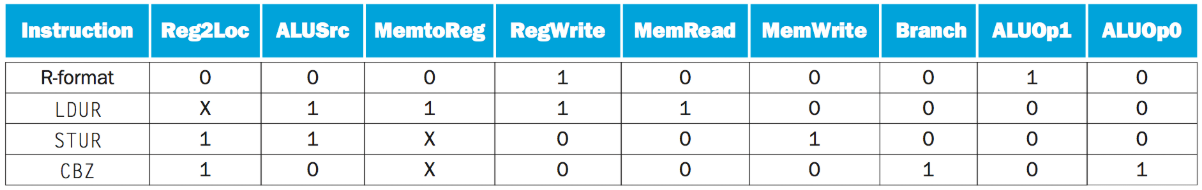
\includegraphics[width=4.75in]{../images/control_value_table.png}
	\end{center}
\end{figure} 

\section{Control Unit Test}
The Control Unit is crucial to operation of your datapath, so it needs to be tested thoroughly.  Every supported instruction (listed above) should be tested with the Control Unit Test.  To facilitate testing, I have provided an Expected Results Table with 10 instructions listed across the top (ARM-Lab/testfiles/ExpectedResultsTable.xlsx).  These are the instructions that you should use to test your Control Unit and your full Decode stage (once we finish it).  The rows of the table are signals that will be inputs and outputs of the control module.  

Before writing your unit test, you should fill in every cell in this table with the expected results.  This includes producing the machine code for each instruction.  Then, use the necessary bits of these machine code instructions as inputs to your Control Unit Test and verify the outputs.  You should display the outputs on your simulation results in the same order that they are shown on the Expected Results Table.  Then, you can go right down the table and easily verify that your results are correct.  

Save the Expected Results Table on GitHub, because we will be adding to it in future labs.  Note that for this lab, you do not need to have time values at the top of your expected results tables.  The instructions give us sufficient granularity.

Note that, at this point, the values that are loaded in the registers do not matter, as we are just testing the Control Unit.  Once we get to the full iDecode stage, we will need to address the register values.

The Verilog implementation between 'if/else' statements and 'case' statements differ.  'If/else' statements will create a series of nested muxes with two inputs each, whereas a case statement will produce one large mux with many inputs.  To maximize speed, we should use case statements. Note that all Verilog case statements must have a default case. But one of the challenges of this lab is dealing with opcodes of different sizes.  Thankfully, Verilog has 'casex', which will only evaluate binary digits that are not labeled X.  So for a CBZ instruction, you can fill in the last 3 digits with XXX and use 'casex'.  The 'casex' syntax will also be very helpful in the Sign Extender.  Also, please create macros in definitions.vh for the opcodes of each instruction and for the ALU Op values of each instruction type.  The values in the macros can include X's when necessary.

\section{Sign Extender}
The final major component of the Decode stage is the Sign Extender.  The Sign Extender should use information in the instruction to create a 64-bit output value to use as an address or branch offset.  You need to extract the constant value from the instruction (this will be different for each instruction type), place that extracted value in the least significant bits of the sign\_extended\_output, then sign extend that value.  For positive values, the sign extender should fill extended bits with 0s.  For negative values, the sign extender should fill the extended bits with 1s.  The sign extender should support extending address values from the following instructions:
\begin{enumerate}
	\item LDUR
	\item STUR
	\item CBZ
	\item B
\end{enumerate}

\section{Sign Extender Test}
The Sign Extender Test should utilize the instructions from the Control Unit test.  Verify that your Sign Extended Output on the Simulation Results matches the value on your Expected Results table.  Instructions that don't use a Sign Extended Output (like R-Type) should fall into the default case.  Fill in the Expected Results Table with the default value.   Note that for this lab, you do not need to have time values at the top of your expected results tables.  The instructions give us sufficient granularity.

\clearpage
\section{Your Assignment}

You are to:
\begin{enumerate}
\item Fill in the entire Expected Results Table, starting with the version that I provide in the testfiles section in GitHub.
\item Create a Control Unit module.
\item Create a Control Unit Test and verify that the simulation results match your Expected Results Table.
\item Create a Sign Extender module.
\item Create a Sign Extender Test Module and verify that the simulation results match your Expected Results Table.
\item  Write a lab report according to the LabN format.
\end{enumerate} 